%----------------------------------------------------------------------------------------
%    PACKAGES AND THEMES
%----------------------------------------------------------------------------------------

\documentclass[aspectratio=169,xcolor=dvipsnames]{beamer}
\usetheme{SimplePlus}

\usepackage{hyperref}
\usepackage{graphicx} % Allows including images
\usepackage{booktabs} % Allows the use of \toprule, \midrule and \bottomrule in tables

%----------------------------------------------------------------------------------------
%    TITLE PAGE
%----------------------------------------------------------------------------------------

\title{Cubical Complexes}
\subtitle{}

\author{Enei Sluga, Simon Hehnen}

\institute
{
    Faculty of Computer and Information Science \\
    University of Ljubljana % Your institution for the title page
}
\date{\today} % Date, can be changed to a custom date

%----------------------------------------------------------------------------------------
%    PRESENTATION SLIDES
%----------------------------------------------------------------------------------------

\begin{document}

\begin{frame}
    % Print the title page as the first slide
    \titlepage
\end{frame}

\begin{frame}{Overview}
    \tableofcontents
\end{frame}

%------------------------------------------------
\section{Intdroduction}
%------------------------------------------------


\begin{frame}{Introduction}
    \textbf{What are Cubical Complexes?}
    \begin{itemize}
        \item Cubical complexes are structures built using cubes as building blocks.
        \item They generalize simplicial complexes by using:
        \begin{itemize}
            \item \textbf{0-cubes:} Vertices
            \item \textbf{1-cubes:} Edges (horizontal or vertical)
            \item \textbf{2-cubes:} Squares
        \end{itemize}
        \item Applications in image analysis and higher-dimensional data.
    \end{itemize}
\end{frame}

\begin{frame}{Motivation}
    \textbf{Why Do We Need Cubical Complexes?}
    \begin{itemize}
        \item \textbf{Natural for Grid-Based Data:}
        \begin{itemize}
            \item Many datasets (e.g., images, videos) are naturally structured as grids.
            \item Cubical complexes align directly with pixel/voxel layouts.
        \end{itemize}
        
        \item \textbf{Efficiency in Construction:}
        \begin{itemize}
            \item Avoids the overhead of triangulating grid-based data.
            \item Simple enumeration of cubes with systematic coordinates.
        \end{itemize}
        
        \item \textbf{Applications in Image Analysis:}
        \begin{itemize}
            \item Enables topological analysis of shapes, textures, and regions in images.
            \item Extends to higher dimensions for 3D volumes or dynamic video data.
        \end{itemize}
        
        \item \textbf{A Discrete World}
    \end{itemize}
\end{frame}

%------------------------------------------------

\begin{frame}{Generation of Cubical Complexes}
    \textbf{Steps to Construct Cubical Complexes:}
    \begin{enumerate}
        \item Define a grid structure (e.g., \( n \times n \)).
        \item Assign coordinates to vertices, edges, and squares.
        \item Ensure orientation is consistent (e.g., positive rotational order for squares).
    \end{enumerate}

    \vspace{1em}
    \textbf{Key Feature:} Each cube is labeled systematically for easy computation.
\end{frame}

%------------------------------------------------

\begin{frame}{Example: 2D-Torus}
    \textbf{Generating a 2D-Torus using Cubical Complexes}
    \begin{itemize}
        \item Represent a torus as a 2D grid with periodic boundary conditions.
        \item Connect edges of the grid (left to right, top to bottom).
        \item Visualize the transformation from a grid to a torus shape.
    \end{itemize}

    \vspace{1em}
    \centering
    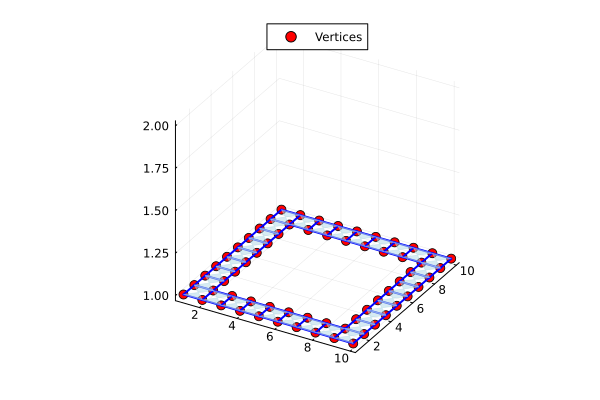
\includegraphics[width=0.5\textwidth]{torus2D.png} % Replace with actual image path
\end{frame}

%------------------------------------------------

\begin{frame}{Example: 3D-Torus}
    \textbf{Generating a 3D-Torus (filled) using Cubical Complexes}
    \begin{itemize}
        \item Represent a torus as a 2D grid with periodic boundary conditions.
        \item Connect edges of the grid (left to right, top to bottom).
        \item Visualize the transformation from a grid to a torus shape.
    \end{itemize}

    \vspace{1em}
    \centering
    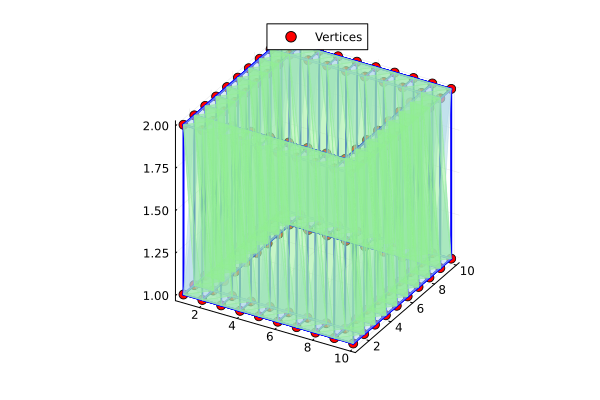
\includegraphics[width=0.5\textwidth]{torus3D.png} % Replace with actual image path
\end{frame}

%------------------------------------------------
\section{Homology}
%------------------------------------------------

\begin{frame}{Homology}
    \textbf{Steps to Compute Homology of a Cubical Complex}
    \begin{itemize}
        \item Define border of a simplex.
        \item Compute the boundary matrix for $n$.
        \item Compute the boundary matrix for $n + 1$.
        \item Simultaneously reduce both matrices.
        \item Compute betti number with rank of reduced matrix
    \end{itemize}
\end{frame}

\begin{frame}{Homology - What's different?}
    \textbf{How is computing homology different in this system?}
    \begin{itemize}
        \item Main difference is in computing the simplex boundary.
        \item Because we construct the cubical complex, we can make sure it's oriented.
        \item We construct the border simplices to follow the same orientation.
        \item Can be very hard as grids produce many simplicies even at small sizes.
    \end{itemize}
\end{frame}

\begin{frame}{Homology Example}
    \textbf{Sphere} - $b_0 = 1, b_1 = 0$
    \vspace{1em}
    \centering
    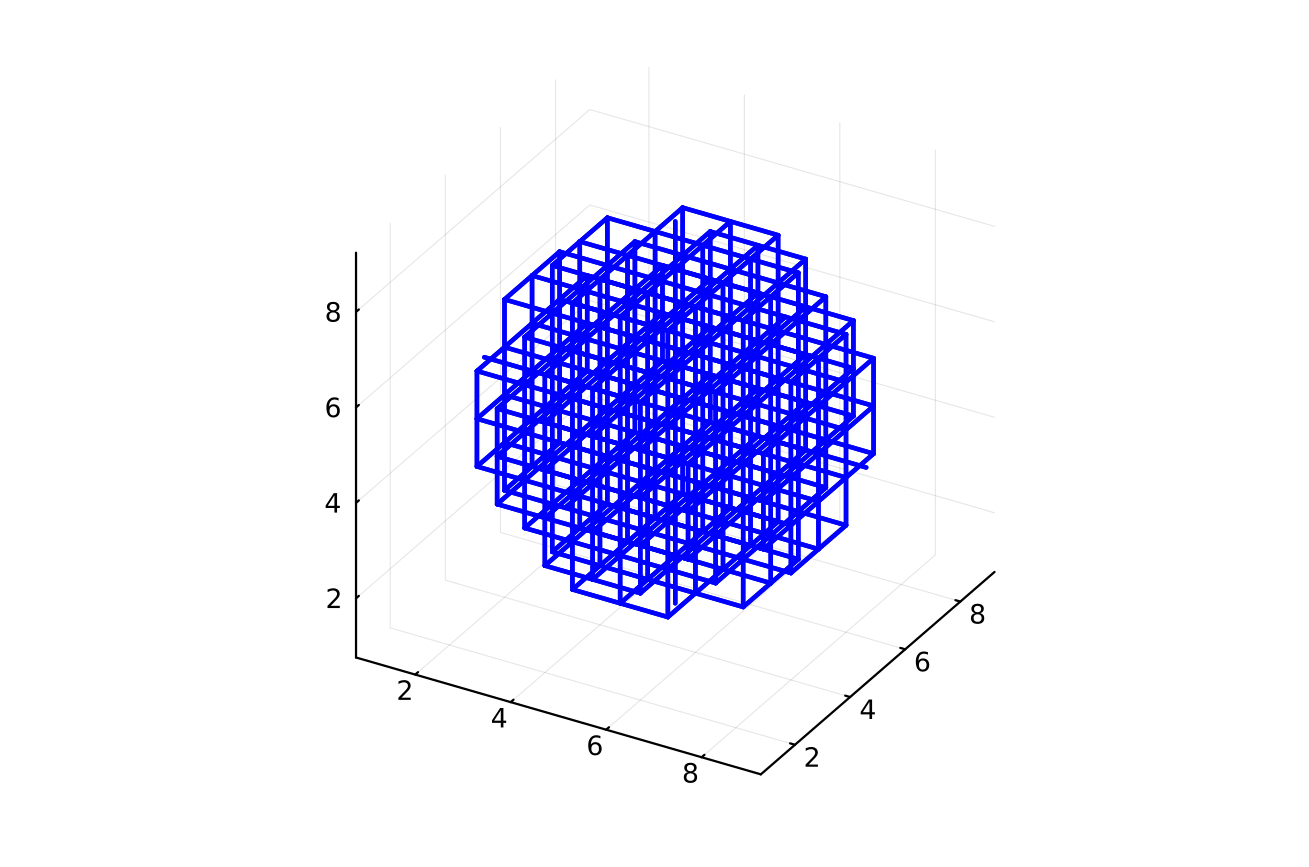
\includegraphics[width=0.5\textwidth]{sphere.png}
\end{frame}

\begin{frame}{Homology Example}
    \textbf{Hollow cube} - $b_0 = 1, b_1 = 0, b_2 = 1$
    \vspace{1em}
    \centering
    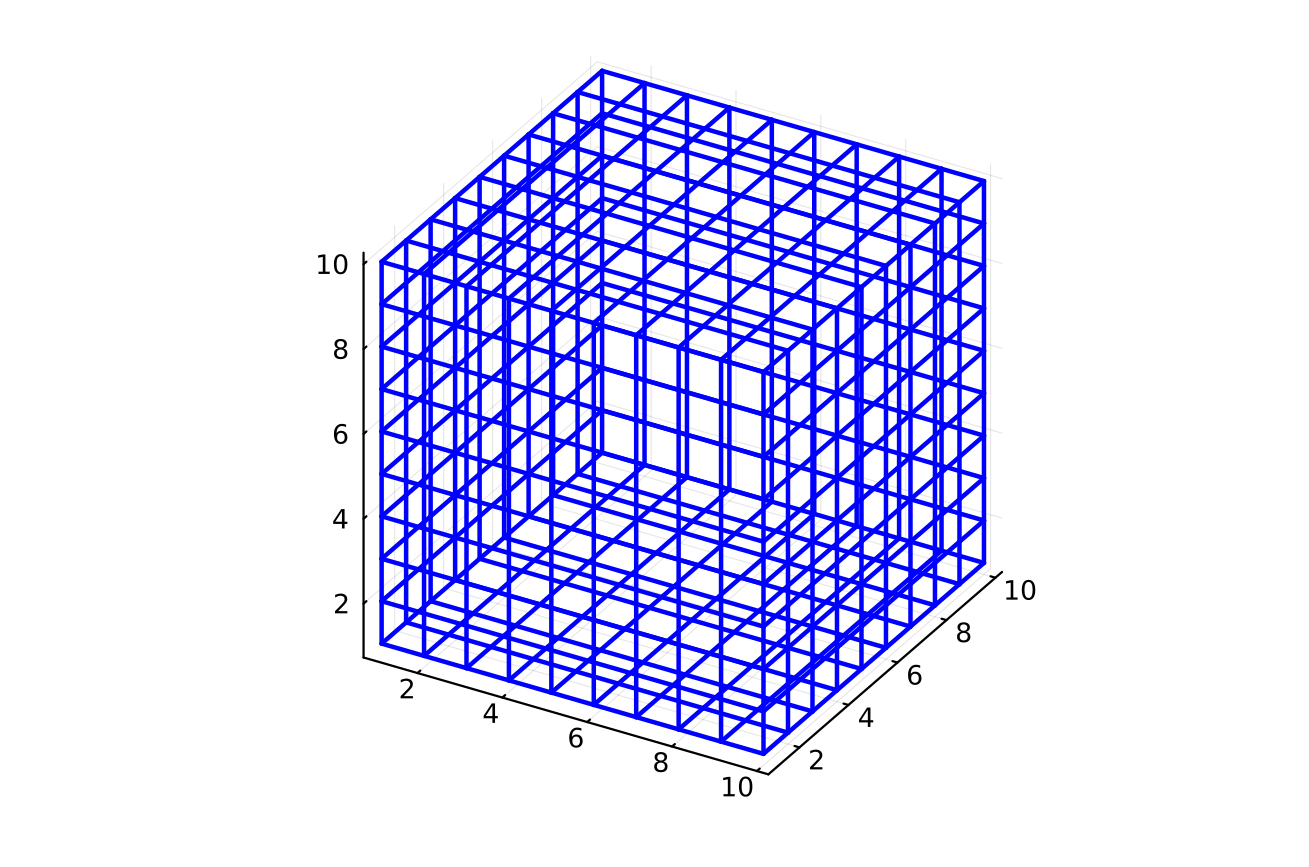
\includegraphics[width=0.5\textwidth]{hollow_cube.png}
\end{frame}

\begin{frame}{Homology Example}
    \textbf{Random grid} - $b_0 = 41, b_1 = 13$
    \vspace{1em}
    \centering
    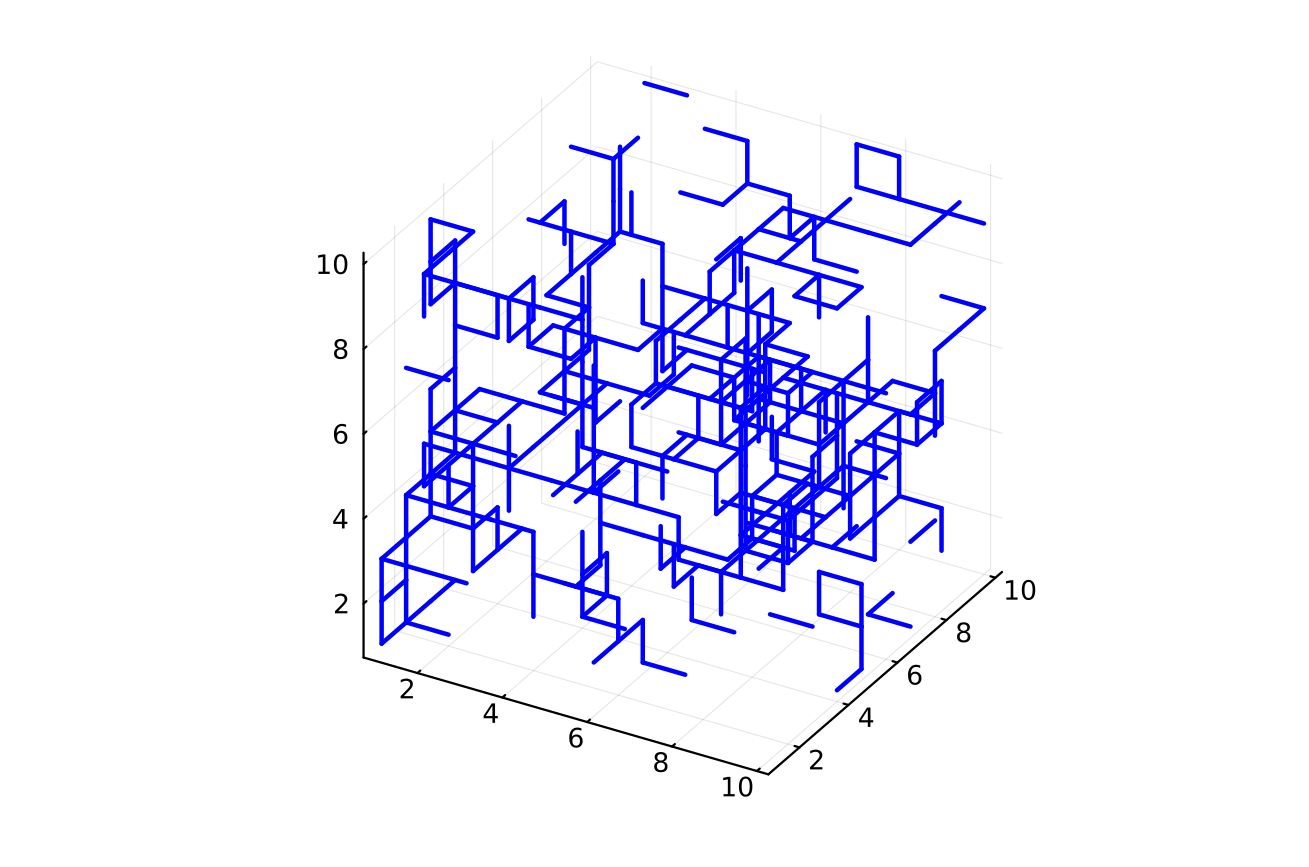
\includegraphics[width=0.5\textwidth]{random_grid.png}
\end{frame}


%------------------------------------------------
\section{Persistent Homology}
%------------------------------------------------


%------------------------------------------------
\begin{frame}{Persistent Homology on Cubical Complexes}
    \textbf{Extending Persistent Homology to Cubical Complexes}
    \textbf{Key Steps:}
    \begin{enumerate}
        \item \textbf{Filtration:} 
        \begin{itemize}
            \item Construct a sequence of subcomplexes \(K_1 \subseteq K_2 \subseteq \dots \subseteq K_n\) by adding cubes based on a threshold (e.g., pixel intensity or distance).
        \end{itemize}
        \item \textbf{Persistence:} Identify when features (e.g., components, loops) are created (birth) and destroyed (death).
        \item \textbf{Output:} Visualize persistence as \textbf{barcodes} or \textbf{persistence diagrams}.
    \end{enumerate}

\end{frame}

%------------------------------------------------
\begin{frame}{Example of Persistent Homology}
    \begin{columns}
        \column{0.5\textwidth}
        \centering
        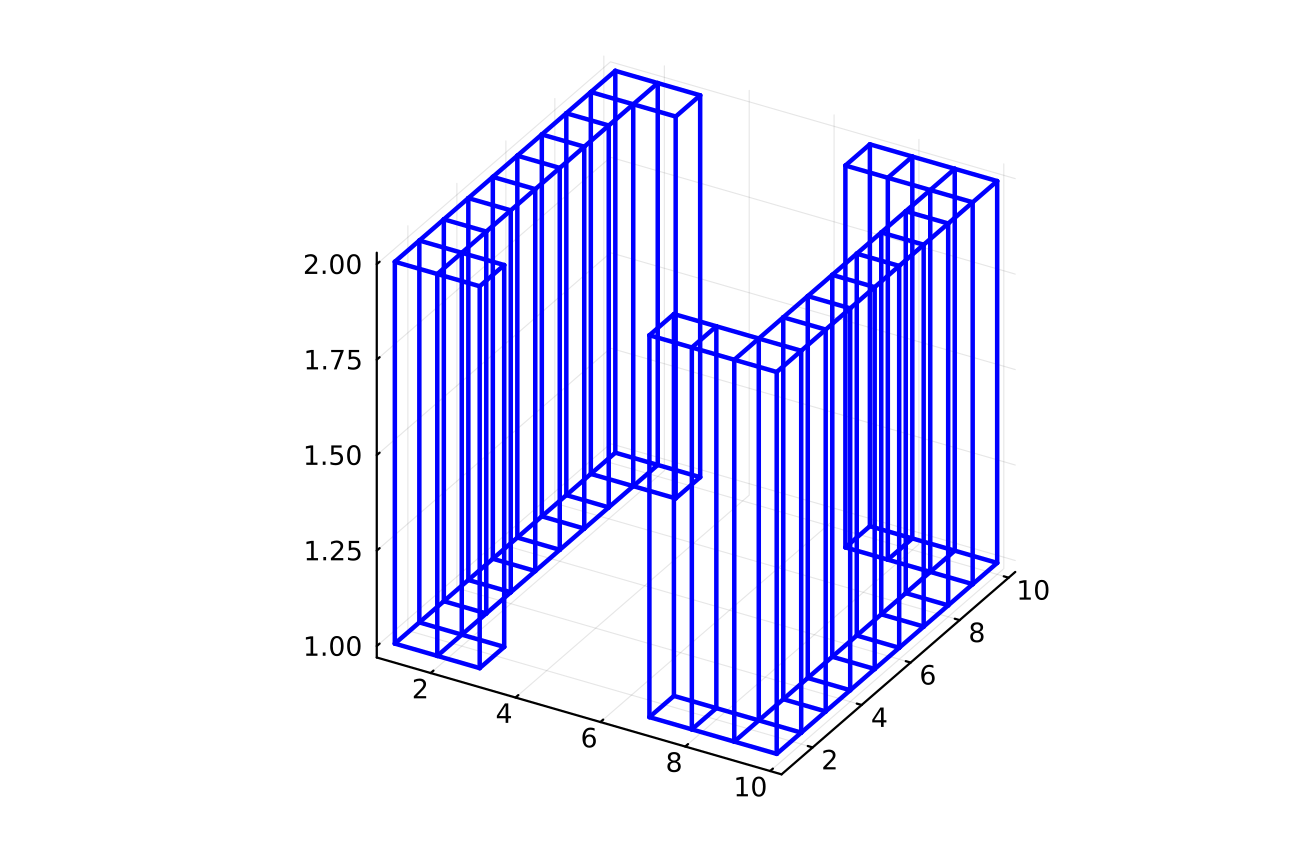
\includegraphics[width=0.4\textwidth]{step1.png}\\
        \vspace{0.5cm}
        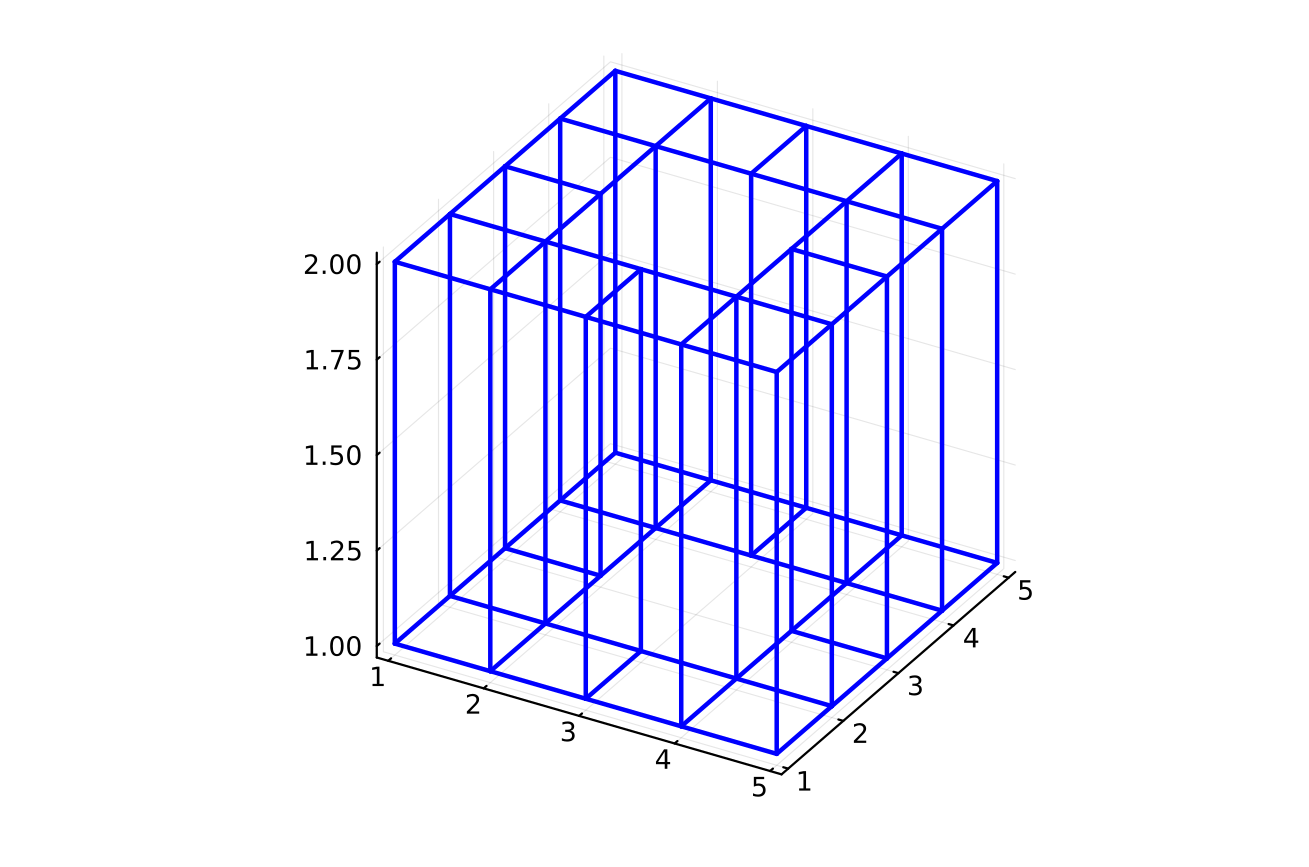
\includegraphics[width=0.4\textwidth]{step2.png}\\
        \vspace{0.5cm}
        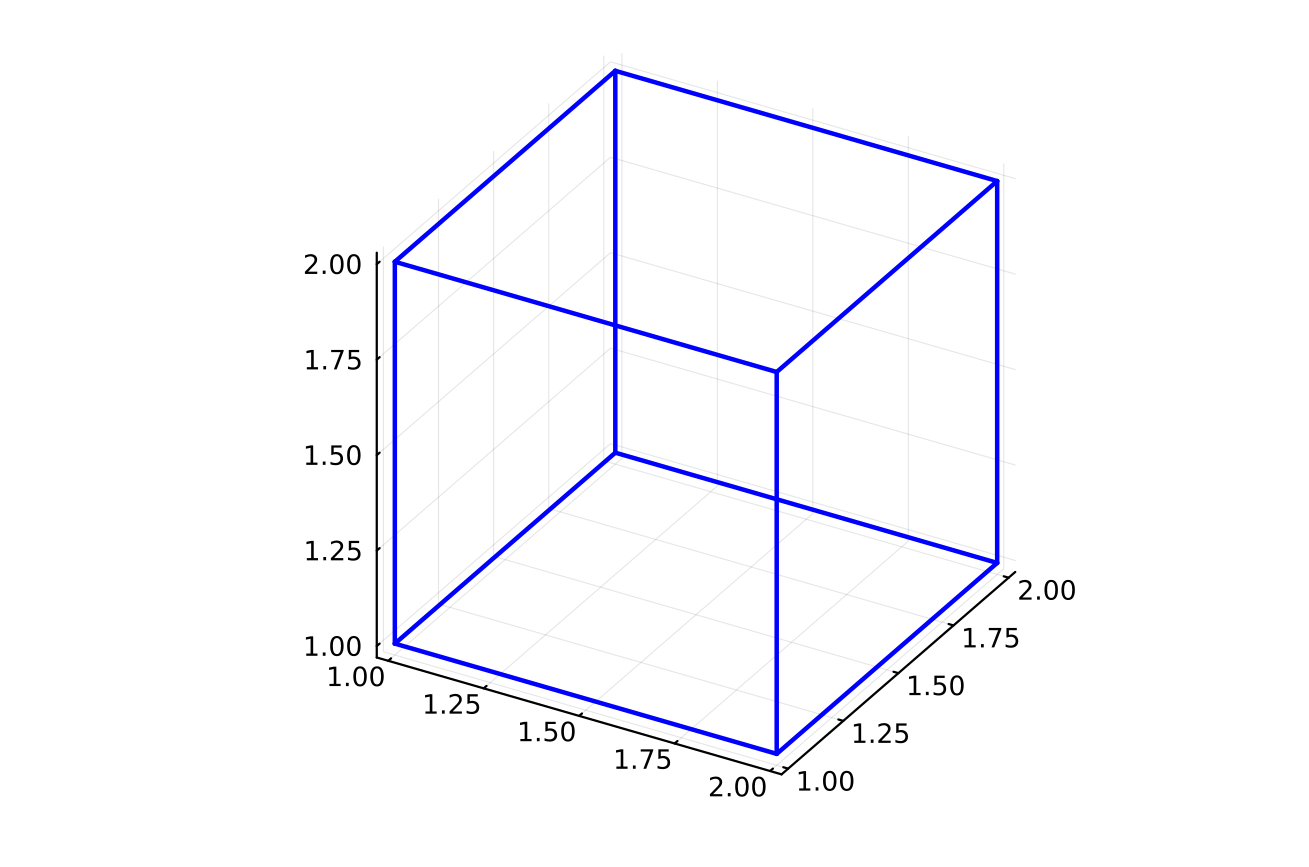
\includegraphics[width=0.4\textwidth]{step3.png}
        
        \column{0.5\textwidth}
        \centering
        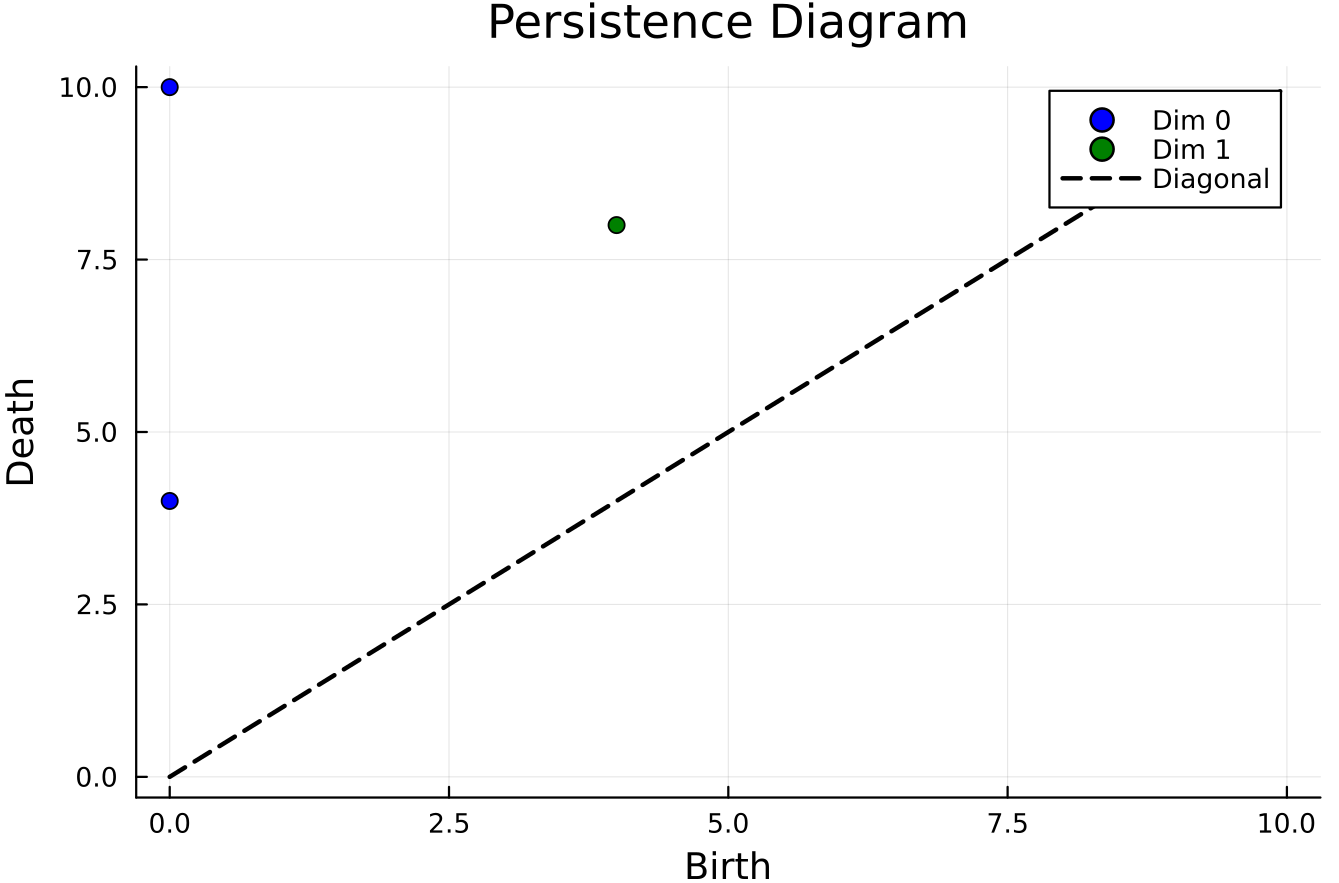
\includegraphics[width=\textwidth]{persistance.png}
    \end{columns}
\end{frame}
%------------------------------------------------


\end{document}